Lo scopo di questo esperimento è valutare la \textbf{limitazione della corrente di uscita} dovuta alla massima corrente erogabile dall’operazionale LM741CN. Il circuito è rappresentato in Figura \ref{fig:Circuito2}. Sono stati utilizzati i seguenti componeneti:
\begin{itemize}
    \item Amplificatore operazionale 741, codice LM741CN
    \item Resistenza di ingresso $R_1=1\text{k}\Omega$, da 0.25W 
    \item Resistenza di uscita $R_2=15\text{k}\Omega$, da 0.25W
    \item Resistenza di carico $R_L=27\Omega$, da 0.25W
\end{itemize}
\begin{figure}[h]
    \centering
    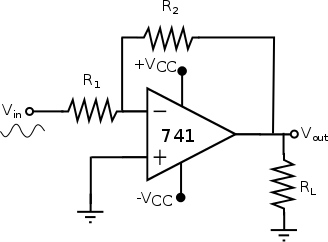
\includegraphics[width=0.5\linewidth]{images/Circuit2.png}
    \caption{Schema circuito}
    \label{fig:Circuito2}
\end{figure}
Il circuito è alimentato dalla tensione duale: $\pm V_{CC}=\pm 10V$.
\subsection{Valutazione del datasheet - prelab}
Sulla base delle informazioni contenute nel datasheet del componente, la massima corrente erogabile dall'amplificatore operazionale LM741CN, a fronte di una alimentazione $\pm V_{CC}=\pm 10V$ , è:
\begin{equation*}
    I_{{out}_{\text{MAX}}}=25mA
\end{equation*}
Da cui si ricava, applicando la legge di Ohm a partire dal valore determinato precedentemente, la massima tensione raggiungibile dall'uscita dell' operazionale:
\begin{equation*}
    V_{{out}_{\text{MAX}}}\approx R_LI_{{out}_{\text{MAX}}}= 0.675V
\end{equation*}
\textit{Nota bene}: il valore della tensione massima è stato trovato applicando la legge di Ohm sulla resistenza di carico. La corrente sulla resistenza di retroazione, essendo dell’odine dei $\mu A$, quindi circa tre ordini di grandezza più piccoli, è stata trascurata.
\subsection{Assemblaggi e settaggi}
Si realizza il circuito il Figura \ref{fig:Circuito2} connettendo opportunamente il generatore di segnali e due canali dell'oscilloscopio; come si vede in figura \ref{fig:LabCircuit2}
\begin{figure}[H]
    \centering
    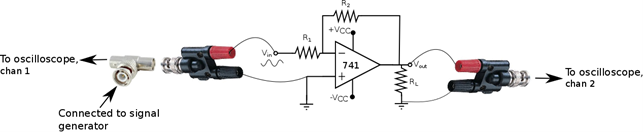
\includegraphics[width=0.9\linewidth]{images/LabCircuit2.png}
    \caption{Collegamento del generatore di funzioni e dell'oscilloscopio}
    \label{fig:LabCircuit2}
\end{figure}
Il generatore di forma d'onda si imposta con le specifiche seguenti:
\begin{itemize}
    \item Forma d'onda: sinusoidale
    \item Ampiezza iniziale: $50mV$ picco-picco
    \item Frequenza: $300Hz$
\end{itemize}
\subsection{Procedura di valutazione e risultati}
Dopo aver acceso l'alimentazione. Si aumenta gradualmente, con step di $10mV$ l’ampiezza della tensione di ingresso, osservando la forma d’onda del segnale di uscita con l’oscilloscopio fino a quando si verifica il clipping del segnale in uscita.\\\\
Alla tensione di $Max V_{out} = 670mV$ si è riscontrato il clipping del segnale.\\\\
In queste condizioni si è calcolato il valore della corrente che scorre sulle resistenze $R_L$ e $R_2$, confrontandolo con il valore massimo della corrente erogabile in uscita dall'amplificatore operazionale. I valori delle correnti sono riassunte nella Tabella \ref{tab:Table2}
\begin{table}[H]
    \centering
    \begin{tabular}{|c|c|}
    \hline
       $Max I_{R_L}=$  & $24.81mA$ \\\hline
       $Max I_{R_2}=$  & $44.67\mu A$ \\\hline
       $Max I_{out}=$ (misurata) & $24.8547mA$ \\\hline
       $Max I_{out}=$ (datasheet) & $25mA$ \\\hline
    \end{tabular}
    \caption{Tabella risultati}
    \label{tab:Table2}
\end{table}
\subsubsection{Conclusioni}
La differenza tra il valore calcolato della corrente massima in uscita con quello fornito dal costruttore può essere dovuta alle tolleranze dei componenti passivi, alla incertezza delle misurazioni e dal particolare chip usato durante l’esperienza.